\chapter{Theory}

Theory relevant to the spectroscopy and detection of single Ba/Ba\textsuperscript{+} in SXe matrices is discussed.  

\section{Ba/Ba\textsuperscript{+} Spectroscopy in Vacuum}

The lowest-lying energy levels for Ba and Ba\textsuperscript{+} are shown in Fig. \ref{fig:elevs}.  For Ba, the main transition is between the ground $6s^{2}$ $^{1}$S$_{0}$ to the excited $6s6p$ $^{1}$P$_{1}$ state.

\begin{figure}[H]
	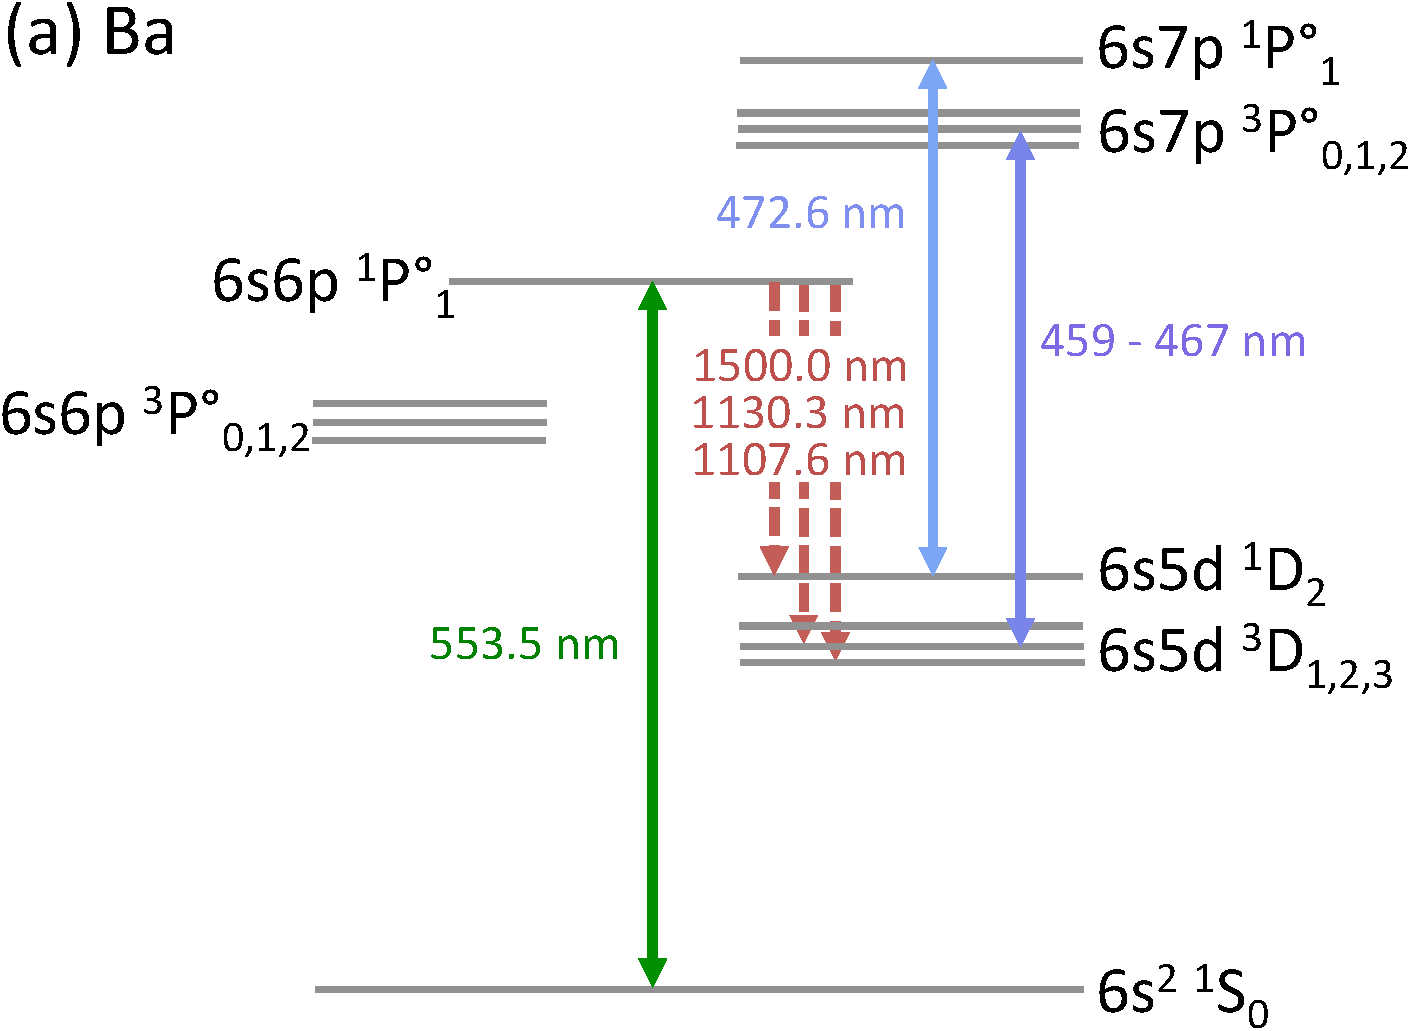
\includegraphics[width=.35\textwidth]{figures/BaLevs_atom.pdf}
	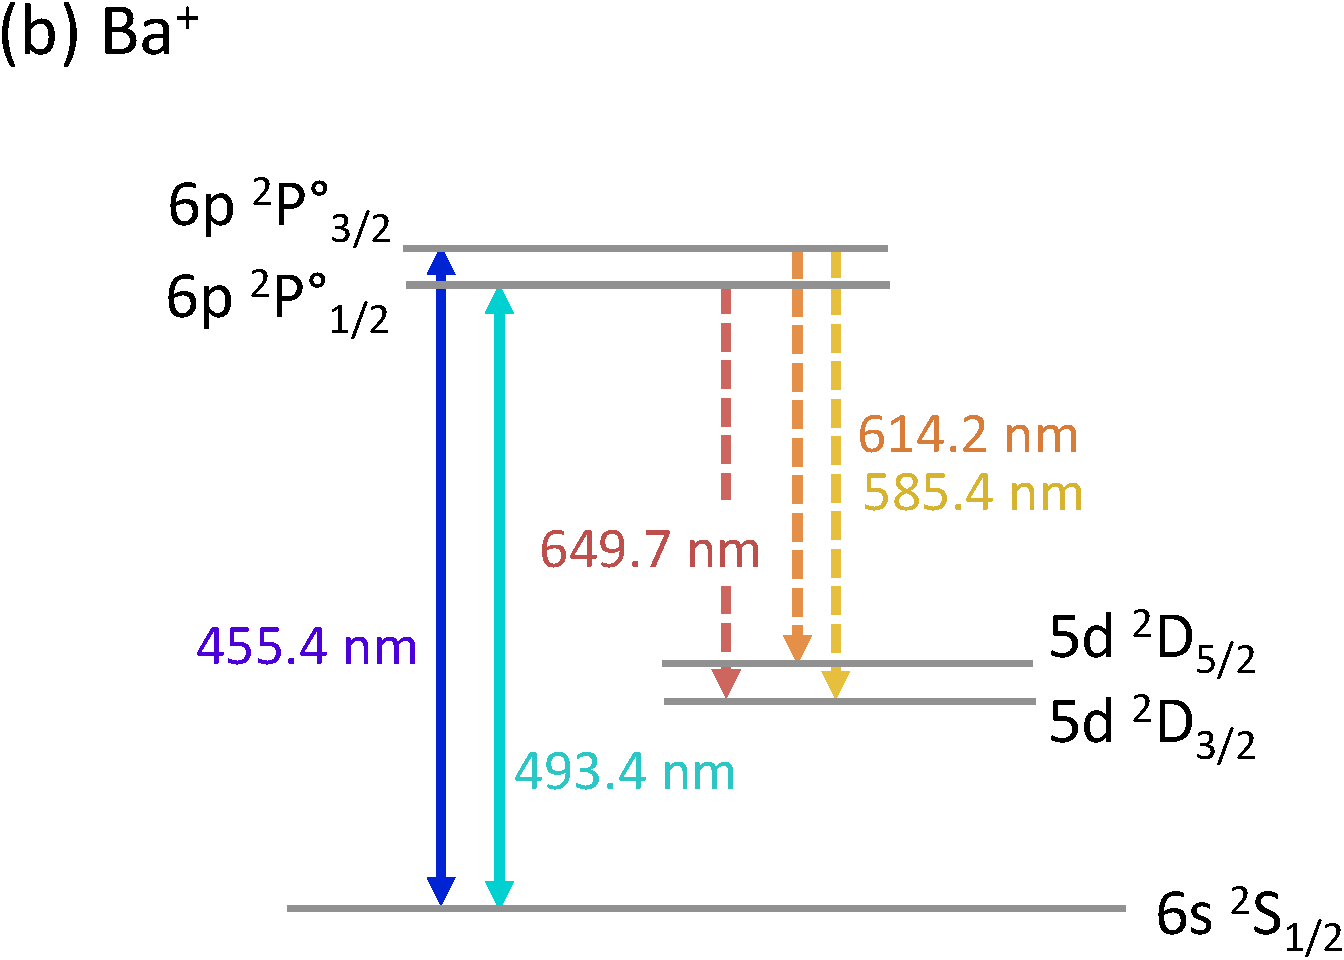
\includegraphics[width=.35\textwidth]{figures/BaLevs_ion.pdf}
	\caption{Energy level diagrams for (a) Ba and (b) Ba\textsuperscript{+} {\color{red}Get rid of high P states in Ba}}
    \label{fig:elevs}
\end{figure}

Single Ba MOT from that paper?  How about single Ba\textsuperscript{+}?

\section{Matrix Isolation Spectroscopy}


